
\section{Building SMBLD: a new parametric dog model}

% Explain why the SMAL parameteric model is unsuitable for the dog category.

At the heart of the method is a parametric representation of a 3D animal mesh, which is based on the Skinned Multi-Animal Linear (SMAL) model proposed by Zuffi et al.~\cite{zuffi2017menagerie}. As discussed in \Cref{chap:cgas}, SMAL is a deformable 3D quadruped mesh parameterized by shape and pose. The \emph{shape}~$\shape \in \R\nshape$ parameters are PCA coefficients of an undeformed template mesh with limbs in default position. The \emph{pose}~$\pose \in \R\npose$ parameters meanwhile govern the joint angle rotations ($35 \times 3$ Rodrigues parameters) which effect the articulated limb movement. The model consists of a linear blend skinning function $F_{v}: (\pose, \shape) \mapsto V$, which generates a set of vertex positions $V \in \RR{3889}{3}$, and a joint function $F_{J}: (\pose, \shape) \mapsto J$, which generates a set of joint positions $J \in \RR{35}{3}$.

\subsection{Introducing scale parameters}

While SMAL has been shown to be adequate for representing a variety of quadruped types, the modes of dog shape variation are poorly captured by the current model. This is unsurprising, since SMAL used only four dogs in its construction.

This is overcome with a simple but effective way to improve the model's representational power over this particularly diverse animal category. The set of shape parameters $\beta$ are augmented with an additional set $\scale$ which independently scale parts of the mesh. For each model joint, parameters ${\scale_x,\scale_y,\scale_z}$ are defined which apply a local scaling of the mesh along the local coordinate $x, y, z$ axes, before pose is applied. Allowing each joint to scale entirely independently can however lead to unrealistic deformations, so scale parameters are shared between multiple joints, e.g. leg lengths. The new Skinned Multi-Breed Linear Model for Dogs (SMBLD) is therefore adapted from SMAL by adding $6$ scale parameters to the existing set of shape parameters. Figure~\ref{fig:shape_variation} shows how introducing scale parameters increases the flexibility of the SMAL model. The original SMAL shape prior is also extended to cover the new scale parameters by fitting SMBLD to a set of $13$ artist-designed 3D dog meshes. 

\begin{figure*}[t!]
    \centering
    % \includegraphics[width=0.23\linewidth]{OllieFigs/mean.png}
    % \includegraphics[width=0.23\linewidth]{OllieFigs/leg_lengthen.png}
    % \includegraphics[width=0.23\linewidth]{OllieFigs/tail_shorten.png}
    % \includegraphics[width=0.23\linewidth]{OllieFigs/tail_puff.png}
    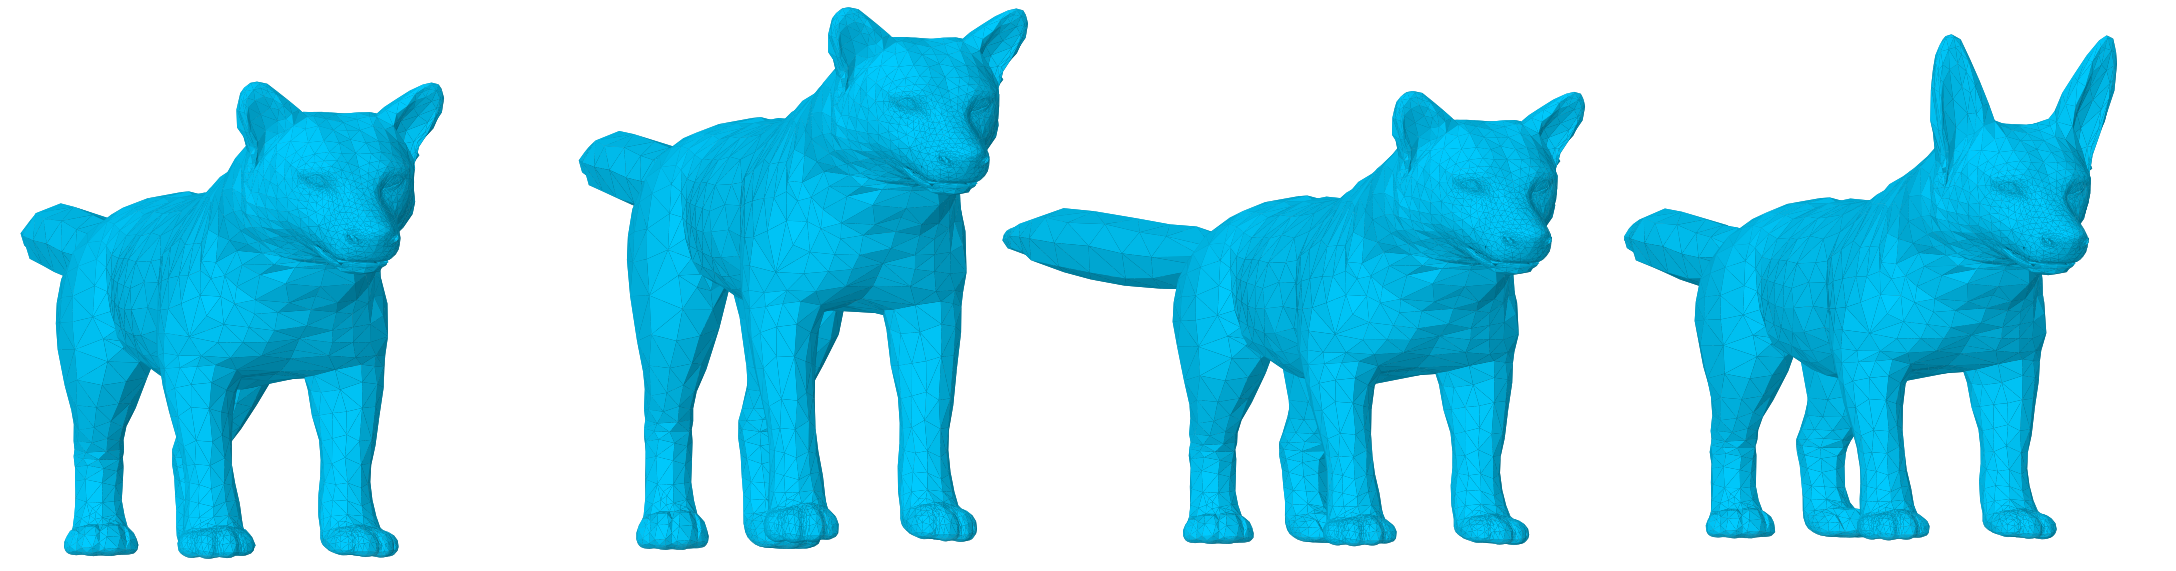
\includegraphics[width=.95\linewidth]{OllieFigs/all_shapevar.png}
    \caption{\textbf{Effect of varying SMBLD scale parameters}. 
    \emph{From left to right}: 
    Mean SMBLD model, 
    25\% leg elongation,
    50\% tail elongation,
    50\% ear elongation.}
    \label{fig:shape_variation}
\end{figure*}

\subsection{Learning a 3D shape prior over scale parameters}

For shape spaces shape space formulations based on principal component analysis (PCA), recall the linear generator function $g: \R{d} \mapsto \R{3n}$ which maps a $d$-dimensional parameter space to $n$ 3D morphable model vertex coordinates: 

\begin{equation}
    g(w) = \bar{c} + Ew
\end{equation}

In this formulation, $\bar{c} \in \R{3n}$ is the mean 3D shape from a training dataset, and $E \in \R{3n \times d}$ is a matrix containing the $d$ most dominant eigenvectors computed over shape residuals $\{c_i - \bar{c_i}\}$. 

% Another hypothesis is that the 3D faces in the reduced parameter space R
% d follow a multivariate normal distribution, which can be directly deduced from the eigenvalues corresponding to E.

%% PCA does assumlaxe normal distribution of features See p.55 SAS book1 or Rummel, 19702 or Mardia, 19793.

A consequence of PCA construction is that the features in the $d$-dimensional parameter space follow a multivariate normal distribution. This can be directly derived from the eigenvalues corresponding to $E$. %% ASK ANDREW, or be less lazy and do the math
With this construction, one can define a likelihood function which measures the probability of a given shape vector $w \in \R{d}$

\begin{equation}
    f(w) = (2\pi)^{-\frac{d}{2}}\det(\Sigma)^{-\frac{1}{2}}e^{-\frac{1}{2}(w-\bar{c})^T\Sigma^{-1}(w-\bar{c})}
\end{equation}

For problems which aim to optimize $w$, the 3D shape prior is obtained by maximizing $f(w)$ or equivalently, by minimizing the negative log likelihood

\begin{equation}
     -\ln\left[f(w)\right] = -\frac{1}{2}\left[\ln\det(\Sigma) + d\ln(2\pi) +  (w - \bar{c})^T\Sigma^{-1}(w-\bar{c})\right]
\end{equation}
and dropping terms with no dependency on $w$ (which remain constant during optimization) leaves the Mahalanobis distance of $w$ to the origin

\begin{equation}
    L(w) = (w - \bar{c})^T\Sigma^{-1}(w-\bar{c})
\end{equation}

% END PRELIMINARIES

% We have already seeen this formulation in Chapter 4.

Another method for improving the generalizability of the SMAL model is to improve the 3D shape prior. Such priors are typically used to ensure shape deformation remain within a realistic and anatomically plausible range. Due to the limited diversity of scans used to build the SMAL model, while the shape prior does enforce realism among deformations, it does not allow for a wide enough range to cover the set of dogs in our dataset.

We improve the quality of the prior (and learn a prior over our new scale parameters) by fitting to a set of $13$ artist-designed 3D dog meshes, designed for animation use, which are more varied than the original set. We apply an energy minimization scheme which aligns the SMAL vertices to each scan, under smoothing regularizers.

Recall that SMBLD is adapted from the SMAL~\cite{zuffi2017menagerie} deformable animal mesh, by including limb scaling parameters. We learn a prior by fitting our SMBLD model, which comprises parameters for pose $\pose$ and shape $\beta$ (the latter of which includes our scaling parameters $\kappa$).

Note that fitting SMBLD to 3D scans is significantly easier than to 2D images, since the complete 3D information of the target mesh is available. In addition, our target meshes are not particularly detailed and are already aligned in T-pose, so we avoid need for a complex alignment technique as discussed in, for example SMPL~\cite{loper15smpl} or SMAL~\cite{zuffi2017menagerie}.

We run an energy minimization process to align the SMBLD mesh to the 3D scans, subject to some smoothing regularizers. We minimize the following energy formulation:

\begin{equation}
    \E{opt} = \E{chamfer} + \E{laplacian} + \E{edge} + \E{normal}
\end{equation}
where each of these terms has a scalar weight $\lambda$. We set $\W{chamfer}=\W{edge}=1.0$, $\W{normal}=0.01$ and $\W{laplacian}=0.1$. We run the optimization using SGD, learning rate $1.0e^{-4}$ for $1000$ iterations.

\ss{Chamfer energy.} A measure of the average distance between vertices of the SMBLD mesh $V=F_v(\pose, \shape)$, and the target mesh vertices $V'$, when $p$ vertices $v_{i}, v'_{j}$ are sampled from each mesh respectively:
\begin{equation}
        \E{chamfer}(V, V') = \frac{1}{p} \sum_{i=1}^p \min_j^p  \left | v_{i} - v'_{j} \right |
\end{equation}

\ss{Uniform laplacian energy.} A measure of the mesh smoothness.

\ss{Edge energy.} This energy is equal to the average edge length across the mesh, and is used to encourage uniform distribution of vertices.

\ss{Normal energy.} This energy promotes consistency between adjacent faces. It is a measure of the average normal consistency between adjacent faces. For two faces with normals $\mathbf{n_0}$ and $\mathbf{n_1}$, the normal consistency is $1 - \frac{\mathbf{n_0} \cdot \mathbf{n_1}}{\left|\mathbf{n_0}\right|\left|\mathbf{n_1}\right|}$.

At the end of this process, we have a collection of fits $\left|(\pose,\shape)\right|_{\{i=1,...13\}}$ from which we can learn our unimodal pose and shape priors. As discussed, we evenutally use this unimodal shape prior to initialize our mixture shape prior, which is tuned with the expectation-maximization step in the training loop.

% \section{Learning mixture shape prior.}
% This section contains additional detail for how we learn our mixture shape prior, using expectation maximization in-the-loop.


% Way more here, and include exampels